\documentclass{beamer}

\usepackage[utf8]{inputenc}
\usepackage{amsmath,amsfonts,amssymb}
\usepackage{graphicx}
\usepackage{tikz}
\usepackage{hyperref}

\graphicspath{{../}{./}{../images/}{./images/}}

% ===== KCPC clean theme (Weeks 1 and 2) =====
\usetheme{default}
\useinnertheme{rectangles}
\useoutertheme{default}
\setbeamertemplate{navigation symbols}{}
\definecolor{kcpc-bg}{RGB}{250,250,250}
\definecolor{kcpc-text}{RGB}{20,20,20}
\definecolor{kcpc-muted}{RGB}{90,90,90}
\definecolor{kcpc-red}{RGB}{176,0,0}
\setbeamercolor{background canvas}{bg=kcpc-bg}
\setbeamercolor{normal text}{fg=kcpc-text}
\setbeamercolor{frametitle}{fg=kcpc-text,bg=kcpc-bg}
\setbeamercolor{title}{fg=kcpc-text}
\setbeamercolor{subtitle}{fg=kcpc-muted}
\setbeamercolor{structure}{fg=kcpc-red}
\setbeamerfont{title}{series=\bfseries,size=\Large}
\setbeamerfont{frametitle}{series=\bfseries,size=\large}
\setlength{\parskip}{0.4em}
\setbeamertemplate{itemize item}{$\rightarrow$}
\setbeamertemplate{itemize subitem}{$\rightarrow$}
\setbeamertemplate{headline}{\vspace{0.2cm}\hspace{0.2cm}\textcolor{kcpc-muted}{\small\insertsection}\hfill}
\setbeamertemplate{footline}{\hspace{0.2cm}\textcolor{kcpc-muted}{\small KCPC}\hfill\vspace{0.3cm}}
\setbeamertemplate{background}{%
  \begin{tikzpicture}[remember picture,overlay]
    \node[opacity=0.035,at=(current page.center)]
      {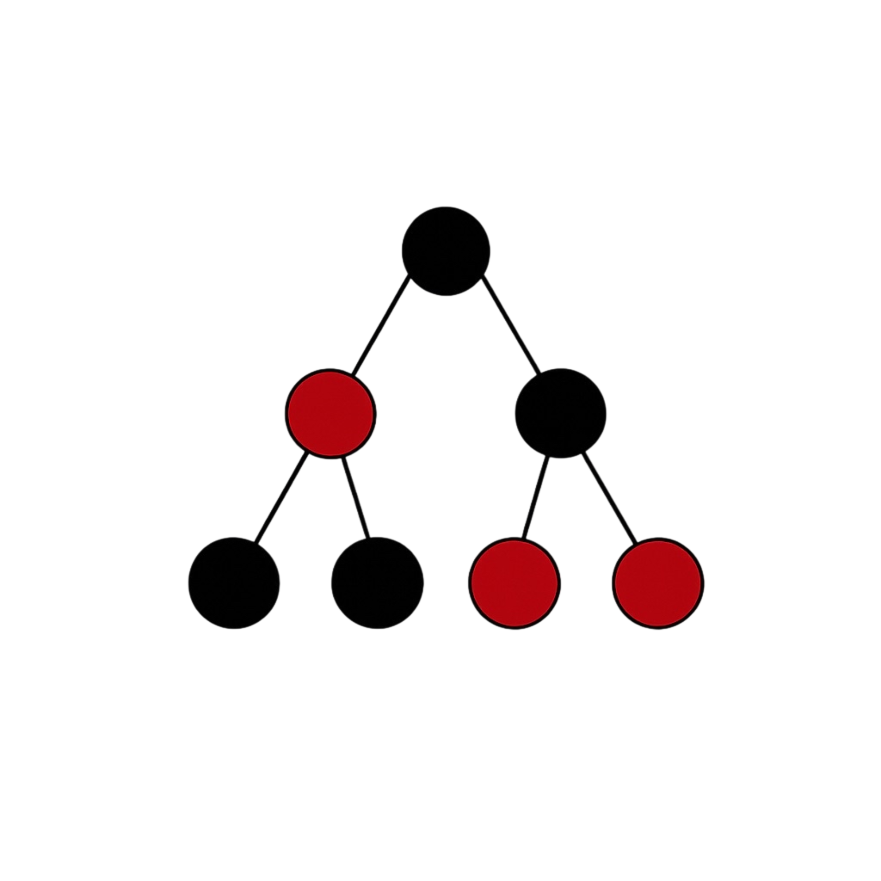
\includegraphics[width=0.55\paperwidth]{kcpc-logo.png}};
  \end{tikzpicture}%
}
\AtBeginSection[]{\begin{frame}[plain]\vfill\centering{\Large\bfseries\insertsection}\vfill\end{frame}}
\hypersetup{colorlinks=true,linkcolor=kcpc-red,urlcolor=kcpc-red}

\title{The Lambda Calculus}
\subtitle{Functions, Computation, and Numbers}
\author{KCPC}
\date{February 5, 2026}

\begin{document}
\begin{frame}[plain]\titlepage\end{frame}

\begin{frame}{Overview}
  \begin{enumerate}
    \item What is the Lambda Calculus?
    \item Syntax of the Lambda Calculus
    \item Alpha and Beta Reductions
    \item Currying
    \item Some Purity
    \item We're Programmers\dots
    \item Some More Complexity
    \item Conclusion
  \end{enumerate}
\end{frame}

\section{What is the Lambda Calculus?}
\begin{frame}{Overview}
  \begin{itemize}
    \item Mathematical language by \textbf{Alonzo Church} in the 1930s
    \item It has no numbers, loops or variables that store values
    \item Can describe any \textbf{computation} done on a computer
  \end{itemize}
\end{frame}
\begin{frame}{Example}
  \[(\lambda f.\lambda x.f(f(x)))\ (\lambda n.n+1)\ 0\]
  \textbf{Evaluates to:} 2

  \textbf{Goal of today:} Understand how this works, and creating our own mathematics!
\end{frame}

\section{Syntax of the Lambda Calculus}
\begin{frame}{What Is a Function?}
  \begin{itemize}
    \item A function takes an \textbf{input}
    \item And produces an \textbf{output}
  \end{itemize}
  \textbf{Mental model:} A function is a machine that takes an input and produces an output.

  \textbf{Important restriction:}
  \begin{itemize}\item In the lambda calculus, a function takes \textbf{one input only}\end{itemize}
\end{frame}
\begin{frame}{Building a Function}
  In the lambda calculus, we build functions using \textbf{abstraction}.
  \[\lambda x.M\]
  \begin{itemize}
    \item The symbol $\lambda$ means ``this is a function''
    \item It tells us that $x$ is an \textbf{input}
    \item Everything after the dot is the \textbf{output rule}
  \end{itemize}
  \textbf{Why do we need $\lambda$?}
  \begin{itemize}
    \item To clearly say when a variable is an input
    \item To avoid confusion between inputs and ordinary names
    \item To make functions precise and unambiguous
  \end{itemize}
\end{frame}
\begin{frame}{Applying a Function}
  Once we have a function, we can apply it to an input.
  \[M\ N\]
  \begin{itemize}
    \item $M$ is a function
    \item $N$ is its input
    \item Application means ``run the machine''
  \end{itemize}
\end{frame}
\begin{frame}{The Three Building Blocks}
  In the lambda calculus, every valid expression is called a \textbf{term}. A term is
  \begin{enumerate}
    \item A variable $x$. A name represents an input.
    \item A function (abstraction) $\lambda x.M$. A function that takes input $x$ and returns $M$.
    \item A function application $M\ N$. Apply the function $M$ to the argument $N$.
  \end{enumerate}
\end{frame}
\begin{frame}{Example: Identity Function}
  \[\lambda x.x\]
  \begin{itemize}
    \item Input: $x$
    \item Output: $x$
    \item \textbf{Interpretation:} return exactly what is given
  \end{itemize}
\end{frame}
\begin{frame}{Functions, Functions Everywhere}
  \begin{itemize}
    \item Every term is built from functions
    \item There are no numbers built in
    \item There is no special logic syntax
    \item In the lambda calculus, everything is a function
  \end{itemize}
\end{frame}

\section{Alpha and Beta Reductions}
\begin{frame}{Alpha Conversion}
  \textbf{Alpha conversion} is:
  \begin{itemize}
    \item The process of renaming a \textbf{bound} variable
    \item Used to avoid confusion or name clashes
  \end{itemize}
  \textbf{General form:}
  \[\lambda x.M\ \longrightarrow_\alpha\ \lambda y.M[y/x]\]
  \textbf{Important rule:}
  \begin{itemize}\item Renaming must not change how the input is used; choose $y$ fresh.\end{itemize}
\end{frame}
\begin{frame}{Alpha Equivalence}
  \textbf{Alpha equivalence} means:
  \begin{itemize}
    \item Two functions are considered the same
    \item If they differ only by input names
  \end{itemize}
  \textbf{Example:} $\lambda x.x\ \equiv_\alpha\ \lambda y.y$

  \textbf{Key idea:}
  \begin{itemize}
    \item Variable names are just labels
    \item What matters is how inputs are used
  \end{itemize}
\end{frame}
\begin{frame}{Beta Reduction}
  \textbf{Beta reduction} is where computation happens.

  Applying a function means: \emph{Replace the input variable with the argument.}

  \textbf{General rule:}
  \[(\lambda x.M)\ N\ \longrightarrow_\beta\ M[N/x]\]
  \textbf{Example:} $(\lambda x.x+1)\ 3\ \longrightarrow\ 3+1\ \longrightarrow\ 4$.

  {\small Substitute only free occurrences of $x$; rename binders first if needed.}
\end{frame}

\section{Currying}
\begin{frame}{Functions Take One Input}
  \begin{itemize}
    \item In the lambda calculus, every function takes \textbf{exactly one input}
    \item There are no two-input or three-input functions
  \end{itemize}
  \textbf{Problem:}
  \begin{itemize}
    \item Many things in maths need more than one input
    \item For example: addition, multiplication
  \end{itemize}
\end{frame}
\begin{frame}{The Idea Behind Currying}
  \textbf{Solution:} A function can return another function.
  \begin{itemize}
    \item First input is given
    \item A new function is returned
    \item That new function waits for the next input
  \end{itemize}
  This idea is called \textbf{currying}.
\end{frame}
\begin{frame}{Currying Explained with Addition}
  In ordinary maths: \[x+y\]
  In the lambda calculus: \[\lambda x.(\lambda y.x+y)\]
  \begin{itemize}
    \item The outer function takes $x$
    \item It returns a new function
    \item The inner function takes $y$
  \end{itemize}
\end{frame}
\begin{frame}{Currying in Action}
  First apply the function to 1:
  \[(\lambda x.\lambda y.x+y)\ 1\ \longrightarrow\ \lambda y.1+y\]
  Then apply the result to 2:
  \[(\lambda y.1+y)\ 2\ \longrightarrow\ 3\]
  \textbf{Conclusion:}
  \begin{itemize}
    \item One input at a time
    \item But still behaves like a two-input function
  \end{itemize}
\end{frame}

\section{Some Purity}
\begin{frame}{Small Issue}
  So far, we've used some notation without actually defining them\dots
  \begin{itemize}
    \item $\lambda x.(\lambda y.x+y)$: what is a ``$+$''?
    \item $(\lambda y.1+y)\ 2\to3$: what is a ``2''? what is a ``number''?
  \end{itemize}
\end{frame}
\begin{frame}{Purest of all Purest}
  \begin{itemize}
    \item Lambda calculus is \emph{pure}, \textbf{pure}
    \item We only have $\lambda$, variables (such as $x$, $y$, etc.), and ``('' and ``)''
    \item We don't have any notion of ``$+$'' or any of the numbers, or even truth values\dots
    \item Let's create them!
  \end{itemize}
\end{frame}

\section{We're Programmers\dots}
\begin{frame}{\dots Bits!}
  \begin{itemize}
    \item Let's begin by defining TRUE and FALSE
    \item Let's give some meaning to these functions
    \item \emph{Foreshadowing\dots{} We will use these definitions to create the operations AND, OR, and NOT}
  \end{itemize}
\end{frame}
\begin{frame}{Some Hint?}
  Think of these two functions:
  \begin{itemize}
    \item $\lambda x.\lambda y.x$
    \item $\lambda x.\lambda y.y$
  \end{itemize}
  What are they? How do they help us?
\end{frame}
\begin{frame}{We Orn’t And}
  Let's try to define these functions which take either a single or two parameters:
  \begin{itemize}
    \item AND: $(x,y)$
    \item OR: $(x,y)$
    \item NOT: $(x)$
  \end{itemize}
\end{frame}

\section{Some More Complexity}
\begin{frame}{Unnaturally Natural Numbers}
  $0,1,2,3,4,5,\dots$ How do we give these ``things'' meaning via lambda calculus?
  \begin{itemize}
    \item Let's define ``zero''
    \item Let's define ``one''
  \end{itemize}
\end{frame}
\begin{frame}{Oh, I Know This!}
  We can use \emph{induction} to continue this pattern and to define all natural numbers. Find the successor function for your numbering system:
  \[\mathrm{SUCC}(n)=n+1\]
\end{frame}
\begin{frame}{Finally Some Mathematics}
  Using what we discovered and learned so far, let's finalise ``our'' mathematics:
  \begin{itemize}
    \item ADD: $(x,y)\mapsto x+y$
    \item SUB: $(x,y)\mapsto x-y$
    \item MUL: $(x,y)\mapsto x\times y$
    \item POW: $(x,y)\mapsto x^y$
    \item DIV: $(x,y)\mapsto x/y$ (if you can do this without looking it up, I'll give you a candy)
  \end{itemize}
\end{frame}

\section{Conclusion}
\begin{frame}{What You've Learned}
  \begin{itemize}
    \item Computation can be built from:
      \begin{itemize}\item Functions\item Substitution\end{itemize}
    \item Numbers are not primitive
    \item Maths and programming meet here
  \end{itemize}
  \textbf{This is also the foundation of functional programming}
\end{frame}

% Answers to the interactive questions above, kept after the original conclusion.
\begin{frame}{Try It Yourself: Booleans (Answers)}
  $\mathrm{T}=\lambda x.\lambda y.x$, $\mathrm{F}=\lambda x.\lambda y.y$;
  $\mathrm{T}\ a\ b\to_\beta a$ and $\mathrm{F}\ a\ b\to_\beta b$.
  \begin{align*}
    \mathrm{AND}&=\lambda p.\lambda q.p\ q\ \mathrm{F},\\
    \mathrm{OR}&=\lambda p.\lambda q.p\ \mathrm{T}\ q,\\
    \mathrm{NOT}&=\lambda p.p\ \mathrm{F}\ \mathrm{T}.
  \end{align*}
  For example, $\mathrm{AND}\ \mathrm{T}\ \mathrm{F}\to_\beta\mathrm{T}\ \mathrm{F}\ \mathrm{F}\to_\beta\mathrm{F}$.
\end{frame}
\begin{frame}{Try It Yourself: Numbers (Answers)}
  A Church numeral $\overline n$ applies a function $n$ times:
  \[\overline0=\lambda f.\lambda x.x,\qquad
    \overline1=\lambda f.\lambda x.f x,\qquad
    \overline2=\lambda f.\lambda x.f(f x).\]
  \[\mathrm{SUCC}=\lambda n.\lambda f.\lambda x.f(n f x)\]
  Thus $\mathrm{SUCC}\ \overline n\ f\ x\to_\beta f(n f x)$, which applies $f$ exactly $n+1$ times.
\end{frame}
\begin{frame}{Try It Yourself: Arithmetic (Answers)}
  {\small
  \begin{align*}
    \mathrm{ADD}&=\lambda m.\lambda n.\lambda f.\lambda x.m f(n f x),\\
    \mathrm{MUL}&=\lambda m.\lambda n.\lambda f.m(n f),\\
    \mathrm{POW}&=\lambda m.\lambda n.\lambda f.\lambda x.n m f x.
  \end{align*}
  They perform $m+n$, $mn$, and $m^n$ iterations respectively. SUB is truncated at zero for Church naturals; DIV additionally requires a zero-divisor convention.
  }
\end{frame}
\begin{frame}{Try It Yourself: Subtraction and Division (Answers)}
  {\small Let $\langle a,b\rangle=\lambda s.sab$ and
  $\mathrm{STEP}\langle a,b\rangle=\langle b,\mathrm{SUCC}\,b\rangle$.
  Iterating STEP $n$ times from $\langle0,0\rangle$ leaves
  $\langle\max(n-1,0),n\rangle$. Hence
  \[\mathrm{PRED}=\lambda n.\mathrm{FIRST}(n\,\mathrm{STEP}\,\langle0,0\rangle),
    \quad\mathrm{SUB}=\lambda m.\lambda n.n\,\mathrm{PRED}\,m.\]
  For $d>0$, DIV iterates $m$ times on a pair $(q,r)$ initially $(0,0)$:
  increment $r$; if $r=d$, reset it to $0$ and increment $q$.
  The invariant after $k$ steps is $k=qd+r$, $0\le r<d$;
  the final $q$ is $\lfloor m/d\rfloor$. Set DIV$(m,0)=0$ by convention.
  See the full lambda-term construction in the solutions sheet.}
\end{frame}

\end{document}
